\subsection{What is a user Interface?}
Wikipedia describes a UI as ' a user interface (UI) is the space where interactions between humans and machines occur'.Common examples of user interfaces in day-to-day life range from the ATM system to The rotary dial developed in 1892(as shown in figure 2.1). The interface creates the link between the user and the devices, A simple user interface is vital and we can notably see this in how we use our devices. Never has there been more variety of interfaces for businesses, consumers, teachers, etc. For example in the early 90s music players were dominated as portable disc players until the early 2000s there were hundreds of different players tailored to your taste and you can decide instead of examples 70s turntables consisting of the needle, arm, and record we are spoilt for variety.
\begin{figure}[h!]
  \centering
    
\includegraphics[width=0.7\textwidth]{Research-Latex/images/classicRotary.jpeg}
     \caption{Classic Rotary Dial  Telephone  .}
\end{figure}


\subsection{Mobile Technologies}
Over the last decade, we have seen a colossal improvement in the connectivity, size, and power of mobile devices. The current trillion-dollar company Apple boosts 'the iPhone in your pocket has more than 100,000 times the processing power of the computer that landed a man on the moon 50 years ago' which is nearly unbelievable.
There are estimated to be a total of 22 billion smart devices on the planet as of the year 2020. As displayed in Fig 2.1 there has been a consistent jump in the popularity of mobile devices or the traditional desktop. There are currently estimated to be 5 million smartphones with android have a share of 75 percent with apple contributing 25 with about  1.2 billion devices.
\begin{figure}[h!]
  \centering
    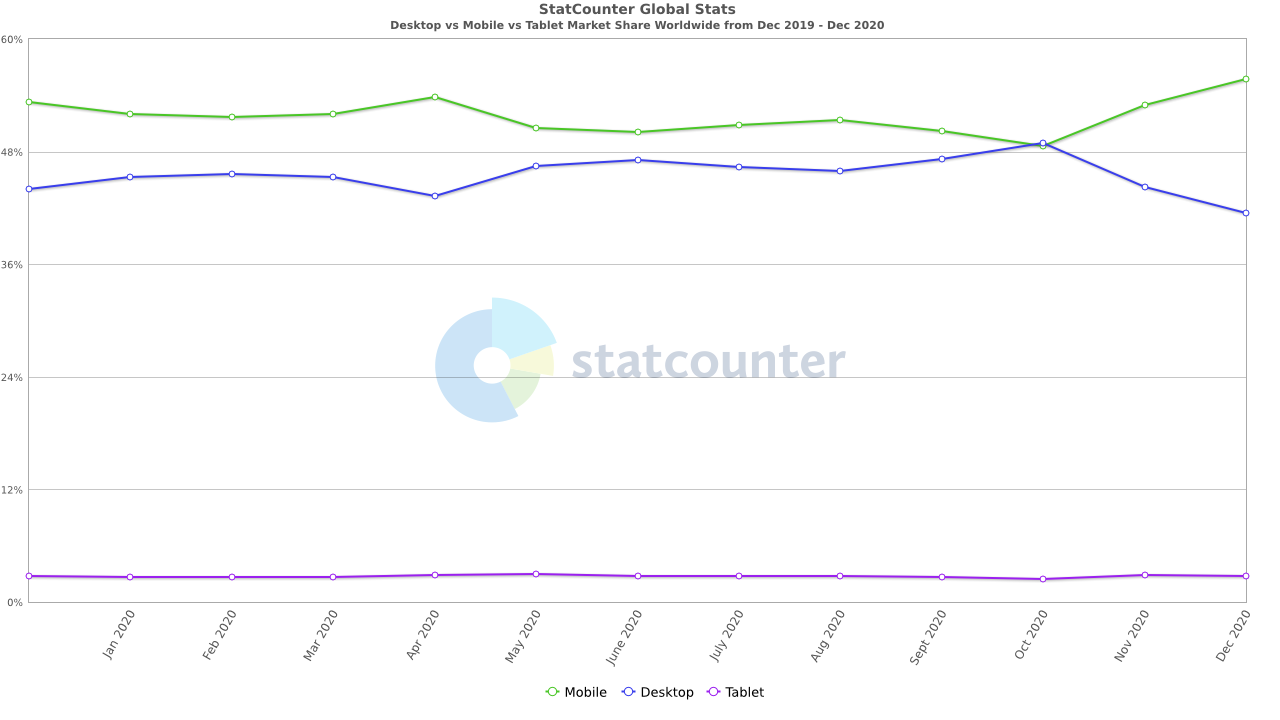
\includegraphics[width=0.7\textwidth]{Research-Latex/images/marketSharePC-Desktop.png}
     \caption{Desktop vs Mobile vs Tablet Global Share .}
\end{figure}

\subsection{Consumer  driven market }

Computing since the early 1960s was only a reality for large companies.The very first consumer orientated computer named 'Altair' developed by Intel in 1974. Today this entry-level Personal Computer would cost an estimated  €15879.44 while today consumers can purchase an entry-level pc such as the Raspberry Pi for €35 which is no larger than the size of a mouse! The editorial team reports 'The Raspberry Pi’s processing speed is approximately 150,000 times faster than ENIAC’s' an unbelievable figure for a machine 30 tons in weight, that is the weight of 15 standard cars! Consumers to a degree dictate what projects large companies deliver yearly

\subsection{The video game Industry  }


The video game industry has been rapidly expanding due to the mainstream use and the expansion of fast and cheaper computer hardware. According to -Statista as of 2019, The video game industry is now the more profitable entertainment industry generating 145.7 billion a year. Due to this explosion in popularity companies have developed new technologies such as Microsoft's project named 'Kinect' in the year 2010. Xbox console users were the first to experience true gesture-based interaction instead of using the console shown in fig 2.1
\begin{figure}[h!]
  \centering
    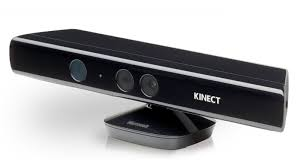
\includegraphics[width=0.5\textwidth]{Research-Latex/images/kinect.jpeg}
     \caption{Kinect Camera Sensor.}
\end{figure}

\subsection{UI hardware}


\textbf{Mouse}\\
Webster's dictionary defines the mouse as follows 'a small mobile manual device that controls the movement of the cursor and selection of functions on a computer display'.The mouse was invented by the 'xerox' company and changed forever how individuals interact with their company when the founder of Apple - Steve Jobs borrowed the device and launched Apple's first Graphical user Interface incorporating the mouse on their newest machine named 'Lisa' on January 19, 1983. The mouse evolved from a simple wired navigation device with a single button now in the year 2020 users have programmable buttons with a light-speed laser tracker like the popular MX-Master developed by Logitech.



\begin{figure}[h!]
  \centering
    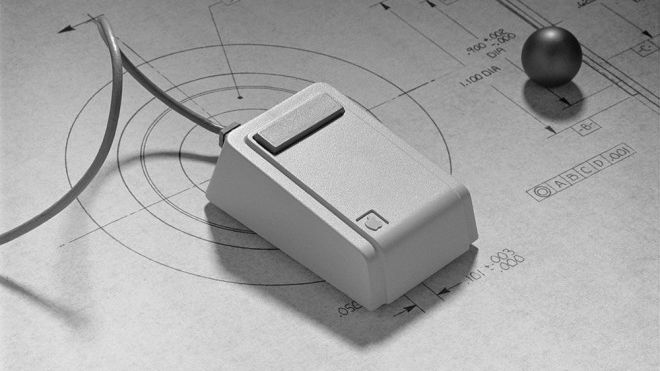
\includegraphics[width=0.7\textwidth]{Research-Latex/images/mouseImage.jpg}
     \caption{Apples Lisa Mouse.}
\end{figure}












\textbf{Keyboard}\\
Websters dictionary defines the keyboard as ' to enter (information) into a computer by using a keyboard'.The keyboard and mouse are the bread and butter of computing.The first keyboard was designed ' In November, 1868 Christopher Latham Sholes [0] and his colleagues, Carlos Glidden, Samuel Willard Soulé, and James Densmore, in Milwaukee shipped out their first 28 key piano style keyboard-like typewriter'.Keyboards are found on all devices such as desktop's to smart which provide a pop digital keyboard using touchscreen capabilities


\begin{figure}[h!]
  \centering
    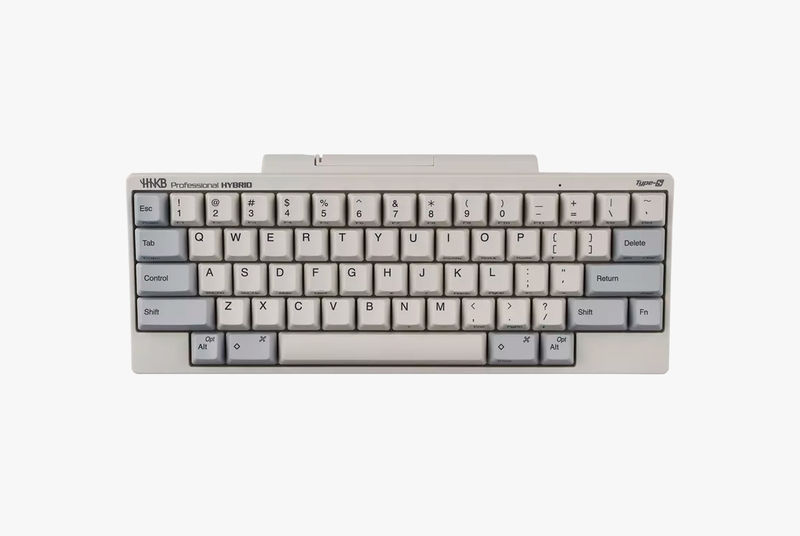
\includegraphics[width=0.4\textwidth]{Research-Latex/images/keyboard.jpeg}
     \caption{Happy Hacking QWERTY Mechanical Keyboard.}
\end{figure}























\textbf{ Command Line Interface vs Graphical User Interface}\\

According to Wikibooks 'A command-line interface or CLI is a method of interacting with a computer by giving it lines of textual commands'.Since the early 1970's computers were devices orientated towards companies and were out of mainstream consumer use. As shown in figure 2.2 there is CLI (command line interface). This method did not implement the mouse and was not operated without a steep learning curve. The CLI dates back to as early as 1950 used on teletype machines. The CLI is still popular today in the tech field but remains for developers and for educational purposes.




\begin{figure}[h!]
  \centering
    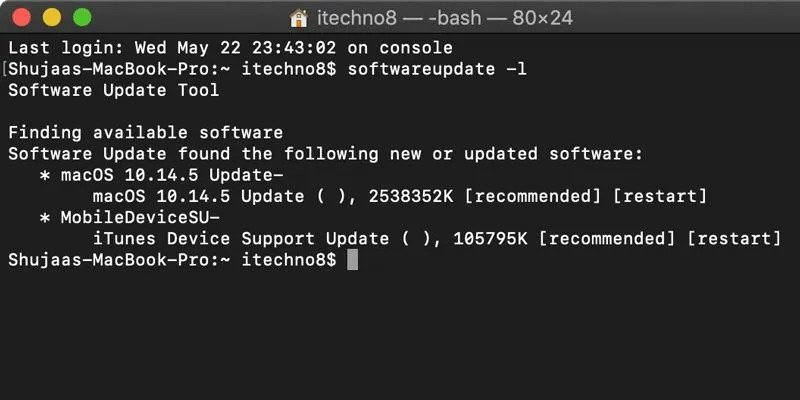
\includegraphics[width=0.7\textwidth]{Research-Latex/images/TheBashterminal.jpg}
     \caption{Bash Terminal on Macintosh Computer}
\end{figure}

GUI (Graphical User Interface) is described by Steven Levy as  'Graphical user interface (GUI), a computer program that enables a person to communicate with a computer through the use of symbols, visual metaphors, and pointing devices'. The 'Xerox Alto' was the first computer to use the graphical user interface over the common text-based command-line interface. In the year 1983 Apple releases the Lisa, the first commercial computer with a graphical user interface (GUI), and changes the norm forever. All commercial computers now use a GUI for some sort such as Windows 10, Mac OSX, and Linux Operating Systems. 

\begin{figure}[h!]
  \centering
    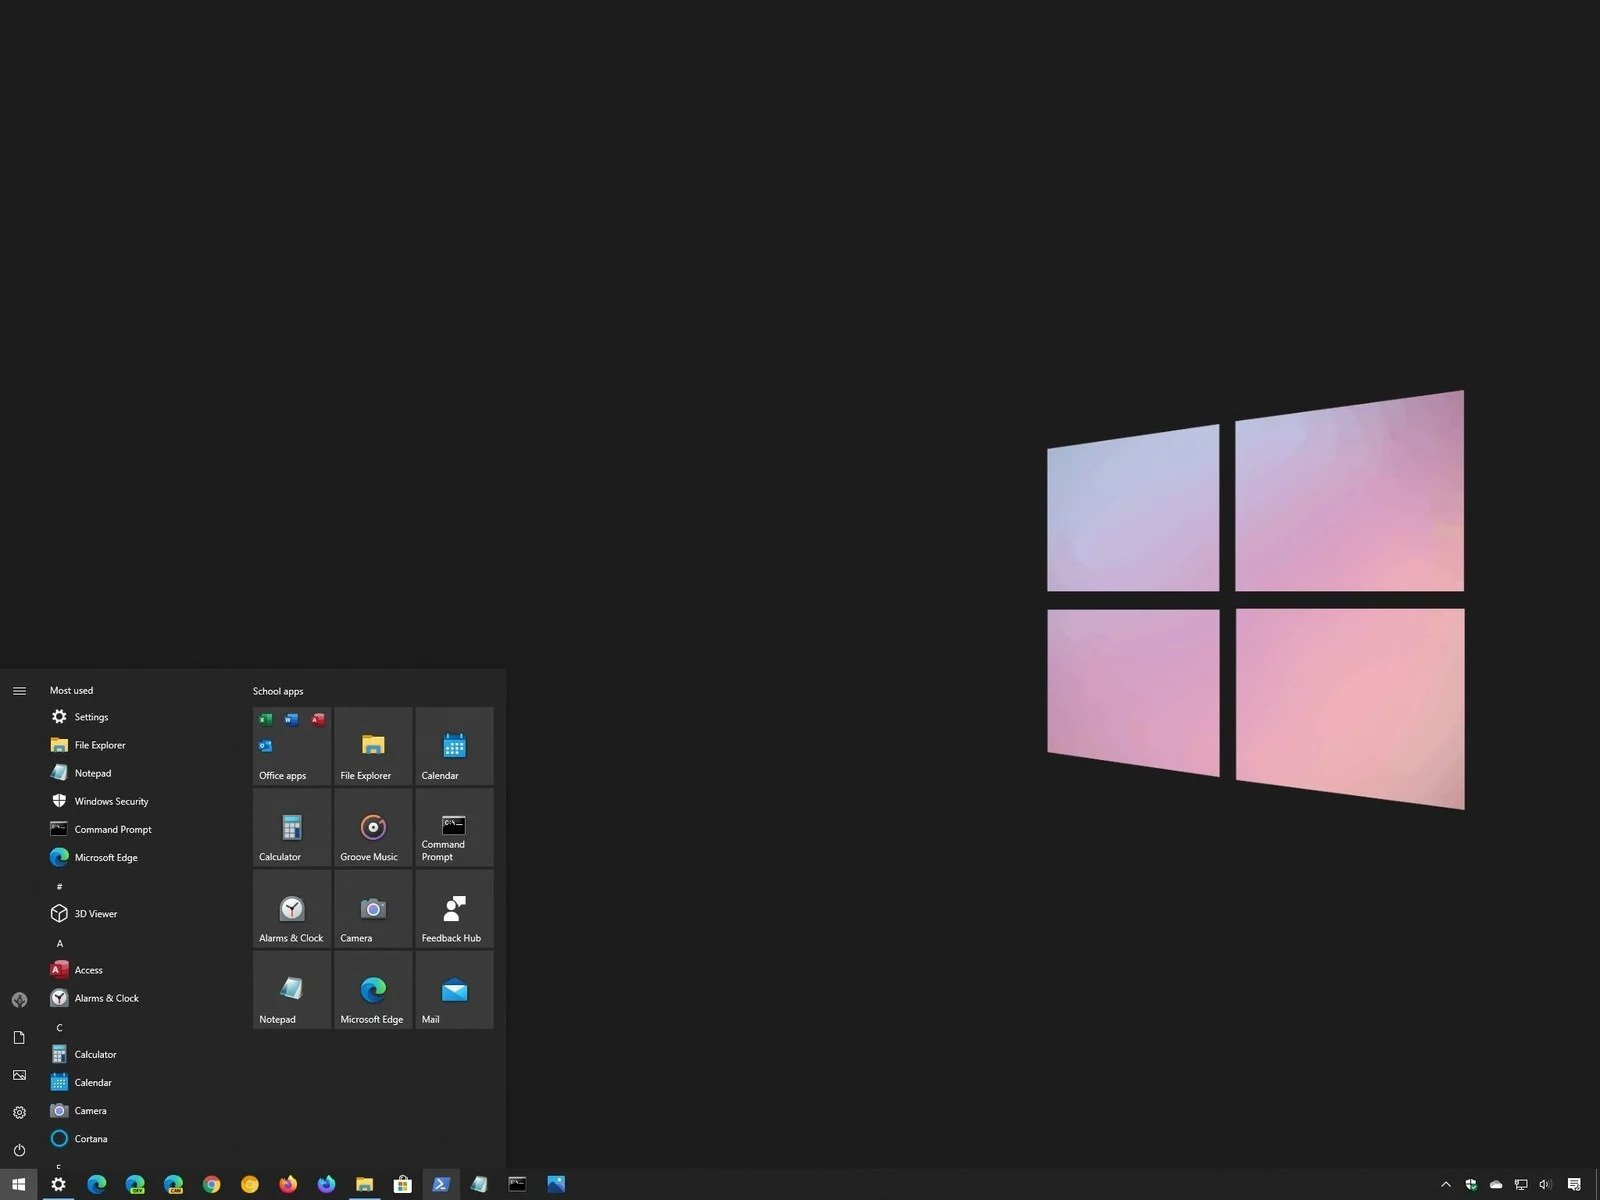
\includegraphics[width=0.7\textwidth]{Research-Latex/images/WINDOWS10-DESKTOP.jpg}
     \caption{Graphical user Interface Windows 10 Desktop.}
\end{figure}






\textbf{Touch Screen}\\

Webster's dictionary defines a touch-screen as ' a display screen on which the user selects options (as from a menu) by touching the screen '.E.A. Johnson developed the touch screen in 1965. It is estimated ' Global Multi-Touch Screen Market Will Reach USD 22.33 Billion By 2025' reported by' Zion Market Research. All smartphones use a touchscreen interface as seen in figure 2.7 the latest generation of the Apple iPad with a full touch screen. Apple launched the Newton—a handheld, portable, touchscreen device—in 1993 but was pulled due to its poor sales and research and development issues. The latest leaps in touch screens jump from the durability named Gorilla Glass to the new 3dimensional touch which allows a new level of features to smart devices using special touch sensors.

 
\begin{figure}[h!]
  \centering
    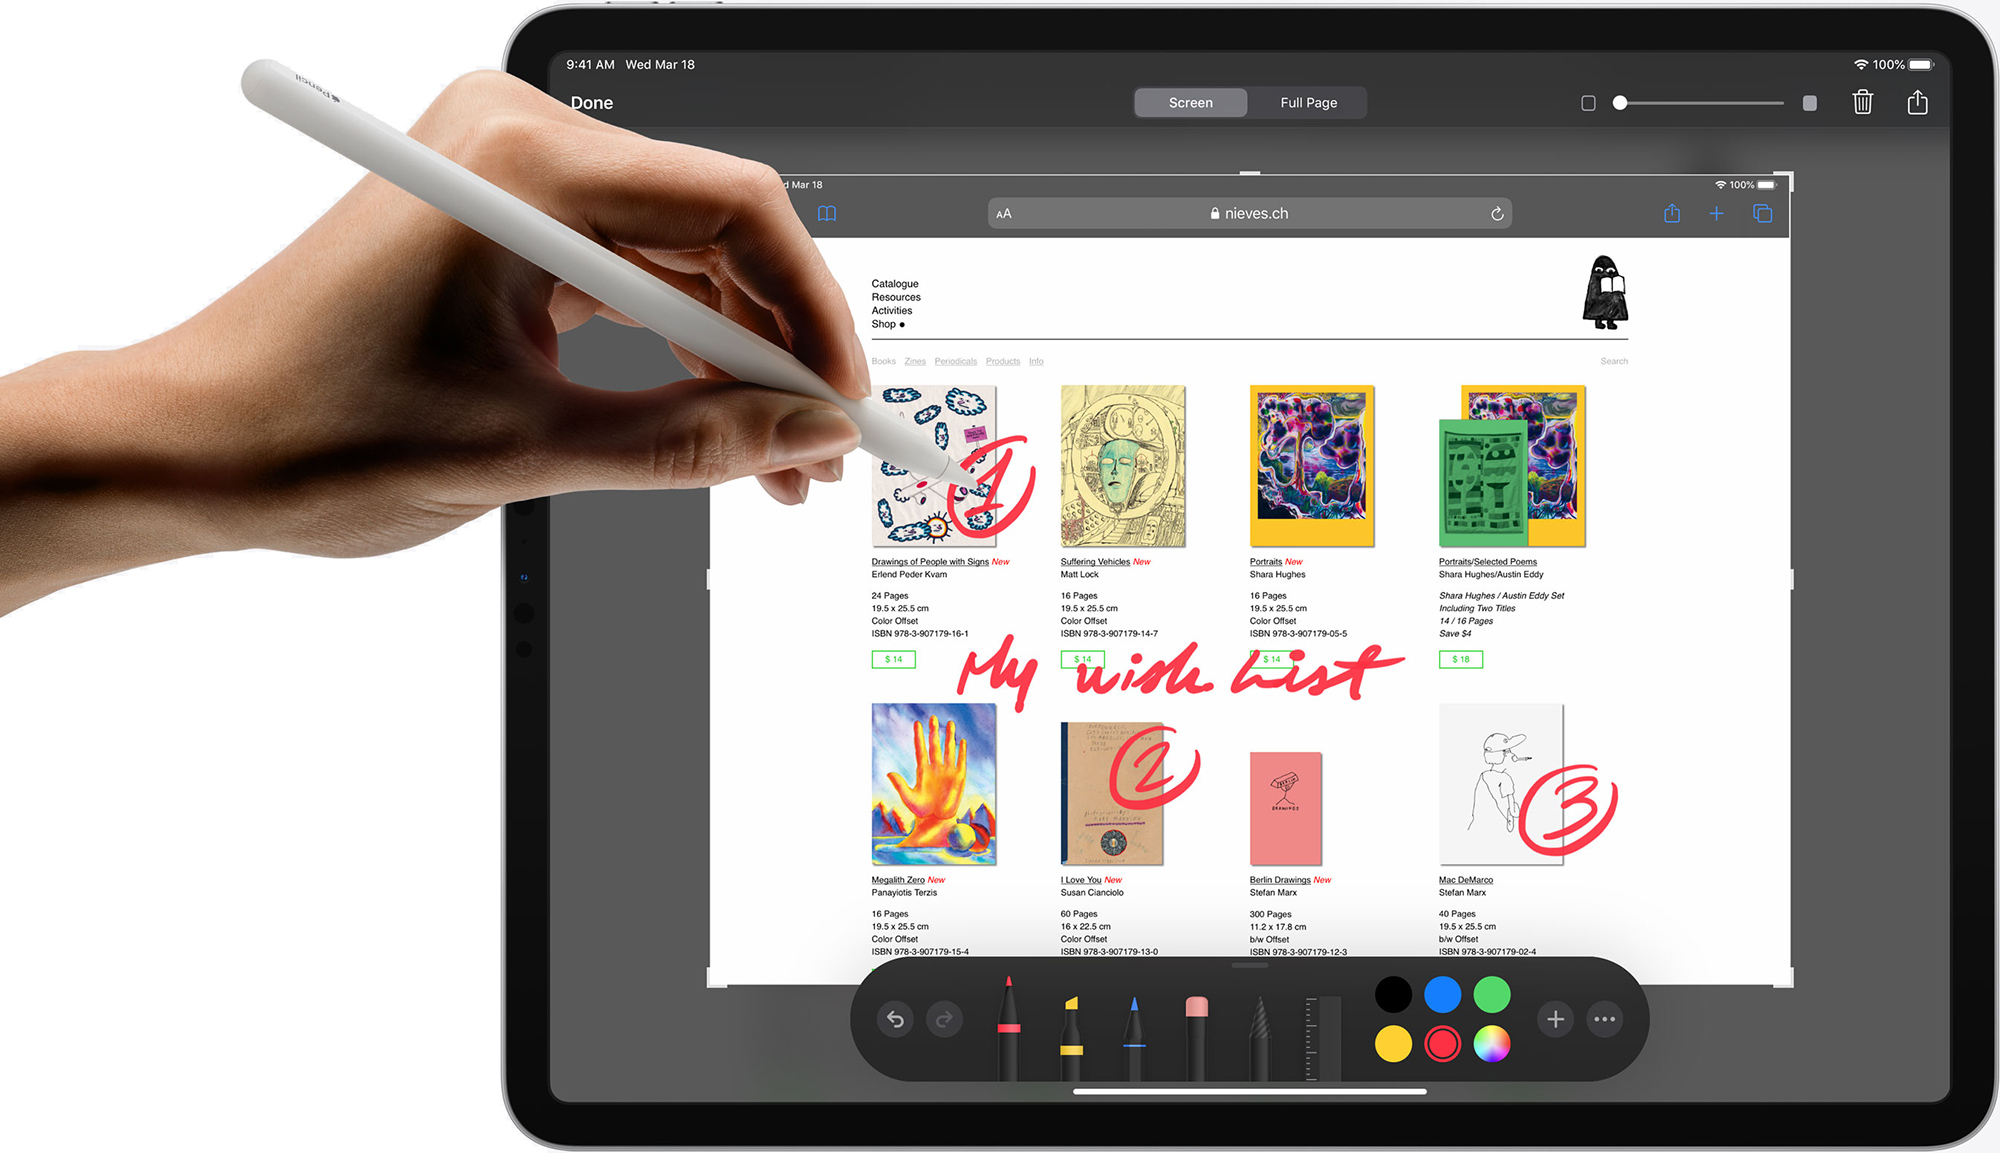
\includegraphics[width=0.5\textwidth]{Research-Latex/images/ipadProTouchScreen.jpg}
     \caption{Apple iPad Pro Touch Screen Tablet }
\end{figure}